\documentclass[a4paper]{article}
\usepackage{subfigure}
%% Language and font encodings
\usepackage[english]{babel}
\usepackage[utf8x]{inputenc}
\usepackage[T1]{fontenc}

%% Sets page size and margins
\usepackage[a4paper,top=3cm,bottom=2cm,left=3cm,right=3cm,marginparwidth=1.75cm]{geometry}

%% Useful packages
\usepackage{amsmath}
\usepackage{graphicx}
\usepackage[colorinlistoftodos]{todonotes}
\usepackage[colorlinks=true, allcolors=blue]{hyperref}

\title{``DOAI: Detecting Objects in Aerial Images''\\
{\em A Proposal for Organizing A Competition on ICPR'2018}}
\author{Gui-Song Xia, Xiang Bai, Serge Belongie, Jiebo Luo, \\ Mihai Datcu, Marcello Pelillo, Fan Hu, Liangpei Zhang}

\begin{document}
\maketitle

\section{Introduction}
Object detection in Earth Vision, also known as {\em Earth Observation and Remote Sensing}, refers to localizing objects of interest (e.g., vehicles and airplanes) on the earth’s surface and predicting their corresponding land-use categories. %It has many applications, such as counting vehicles in parking lot, detecting the dead trees, searching the empty parking space, etc.
The task of object detection in aerial images is distinguished from the conventional object detection task in the following respects:
\begin{itemize}
	\item[-] The scale variations of object instances in aerial images are considerably huge.
	\item[-] Many small object instances are densely distributed in aerial images, for example, the ships in a harbor and the vehicles in a parking lot, as illustrated in Fig.~\ref{fig:samples}.
	\item[-] Objects in aerial images often appear in arbitrary orientations.
\end{itemize}

As is well known to all, datasets have played an important role in data-driven algorithms. Although there exist some datasets in aerial image interpretation, Such as TAS~\cite{TAS}, VEDAI~\cite{VEDAI}, COWC~\cite{COWC} and DLR 3K Munich Vehicle~\cite{DLR3KMunichVehicle}, whereas they only focus on ground vehicles. The UCAS-AOD~\cite{ucas-aod} contains vehicles and planes while HRSC2016~\cite{HRSC2016} only contains ships even though fine-grained category information are provided. All these datasets are less abundant in the number of object classes, which seriously restricts their applicability to complicated aerial scenes. In contrast, NWPU VHR-10~\cite{VHR} is composed of ten different classes of objects while its total number of instances is only around $3000$. A recent effort to ameliorating the lack of data is Spacenet competition, which simply focuses on building and road extraction. However, up to now, a large standard benchmark for common objects detection in aerial images is still lack.

This competition features a new image database of object detection in aerial images. We propose a large-scale dataset with 2000 large-size images ($\sim$4000 $\times$4000), which contain 15 categories and 134,199 instances, each of which is labeled by an arbitrary (8 d.o.f.) quadrilateral. Besides, we propose two tasks for this competition, namely object detection with horizontal bounding box and object detection with oriented bounding box.

Through the dataset and the tasks, we aim to draw attention from the a wide range of communities and call for more future research and efforts on the problems of object dection in aerial images. We believe the competition will not only promote the development of algorithms for object detection in Earth Vision, but also pose interesting algorithmic questions to general object detection
in computer vision.

\section{Dataset and Annotations}

\subsection{Image source}
Image samples in our dataset are collected from multiple sensors and platforms (e.g. Google Earth) with multiple resolutions.

\subsection{Category}
Fifteen categories are chosen and annotated in our dataset, including plane, ship, storage tank, baseball diamond, tennis court, basketball court, ground track field, harbor, bridge, large vehicle, small vehicle, helicopter, roundabout, soccer ball field and basketball court.

\subsection{Annotation method}
In the dataset, each instance's location is annotated by a quadrilateral bounding boxes, which can be denoted as \(\left \{ (x_i,y_i), i=1,2,3,4 \right \}\), where $(x_i, y_i)$ denotes the positions of the oriented bounding boxes' vertices in the image. The vertices are arranged in a clockwise order.
\begin{figure*}[htb!]
\centering
% Requires \usepackage{graphicx}
\subfigure[]{
	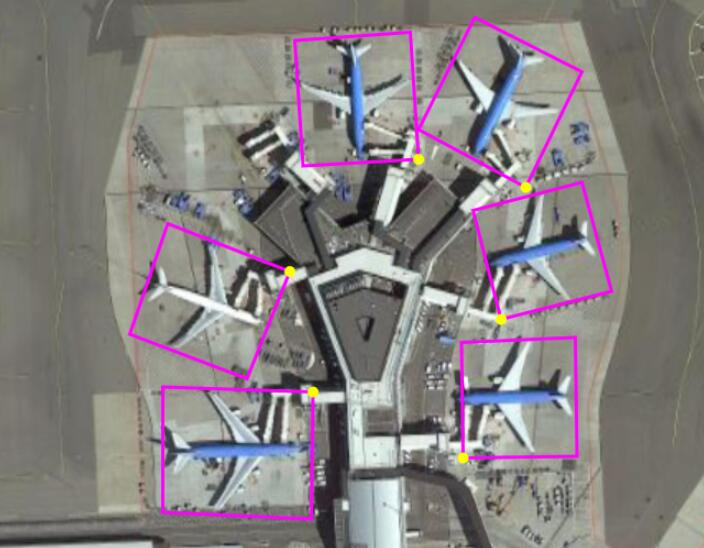
\includegraphics[width=0.2\linewidth]{plane1.jpg}
}
\subfigure[]{
	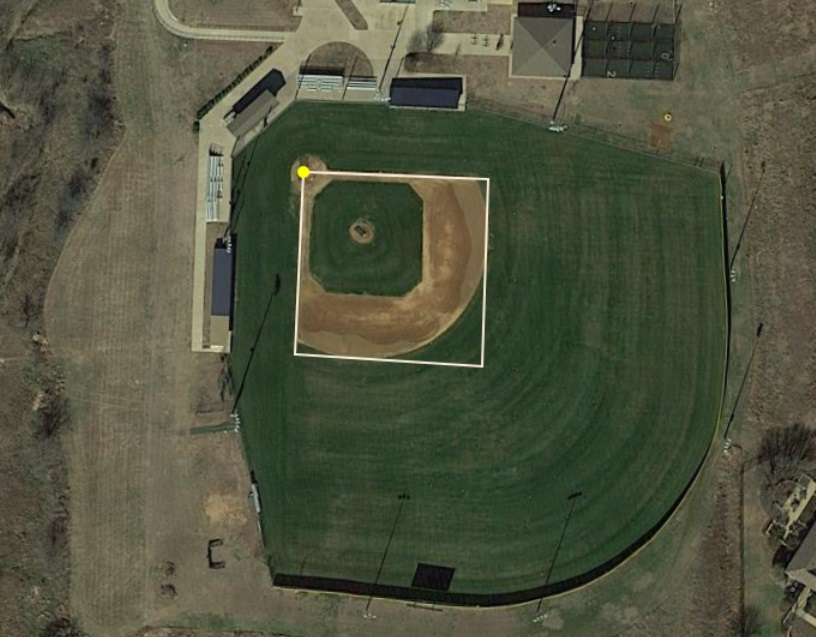
\includegraphics[width=0.2\linewidth]{baseball2.jpg}
}
\subfigure[]{
	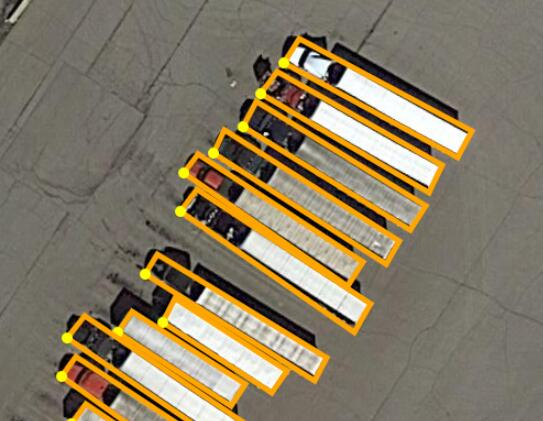
\includegraphics[width=0.2\linewidth]{rotaterec.jpg}
}
\subfigure[]{
	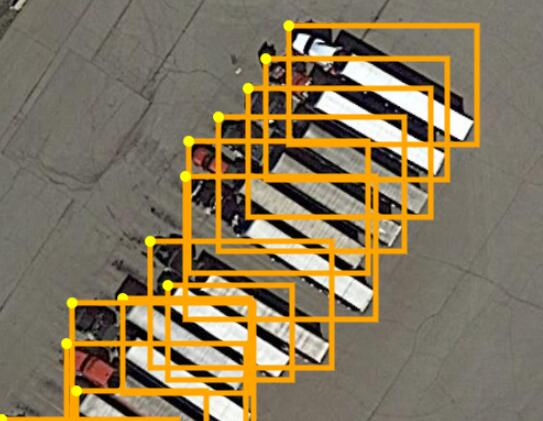
\includegraphics[width=0.2\linewidth]{horizontalrec.jpg}
}
\vspace{-3mm}
\caption{Visualization of adopted annotation method. The yellow point represents the starting point, which refers to:  (a) top left corner of a plane, (b) the center of sector-shaped baseball diamond, (c) top left corner of a large vehicle. (d) is a failure case of the horizontal rectangle annotation, which brings high overlap compared to (c).}
% \caption{(a) The first point $(x_1, y_1)$ \protect (yellow point) indicates the left up of the plane, (b) The first point $(x_1, y_1)$ \protect (yellow point) indicates the center of sector, (c) The first point $(x_1, y_1)$ \protect (yellow point) indicates the left up of the large vehicle. (d) The horizontal rectangle annotation of instances, compare to (c), the overlap between two instance is very high.}
\label{fig:labeing-way}
\end{figure*}

To make a more detailed annotation, as illustrated Fig.~\ref{fig:labeing-way}, we emphasize the importance of the first point \((x_1,y_1)\), which normally implies the “head” of the object. For helicopter,
large vehicle, small vehicle, harbor, baseball diamond, ship and plane, we carefully denote their first point to enrich potential usages. While for soccer-ball field, swimming
pool, bridge, ground track field, basketball court and tennis court, there are no visual clues to decide the first point, so we normally choose the top-left point as the starting
point. As for rounded categories such as roundabout and storage tank, they are annotated with horizontal bounding box, but still the same format of \(\left \{ (x_i,y_i), i=1,2,3,4 \right \}\), where $(x_1, y_1)$ is the top-left point.
Except the annotation of location, category label is assigned for each instance, which comes from one of the above 15 selected categories, and meanwhile a difficult label is provided which indicates whether the instance is difficult to be detected. 
Annotations for an image are saved in a text file with the same file name. At the first line, 'gsd'~\cite{gsd} (ground sample distance, the physical size of one image pixel, in meters) is given.  
From second line to last line in annotation text file, the annotation format is:

$$'gsd': gsd$$
$$x_1^{(1)}, y_1^{(1)}, x_2^{(1)}, y_2^{(1)}, x_3^{(1)}, y_3^{(1)}, x_4^{(1)}, y_4^{(1)}, category, difficult$$
$$x_1^{(2)}, y_1^{(2)}, x_2^{(2)}, y_2^{(2)}, x_3^{(2)}, y_3^{(2)}, x_4^{(2)}, y_4^{(2)}, category, difficult$$
$$...$$

samples of annotated images are shown in Fig.~\ref{fig:samples}

\begin{figure*}[htb!]
\begin{center}
    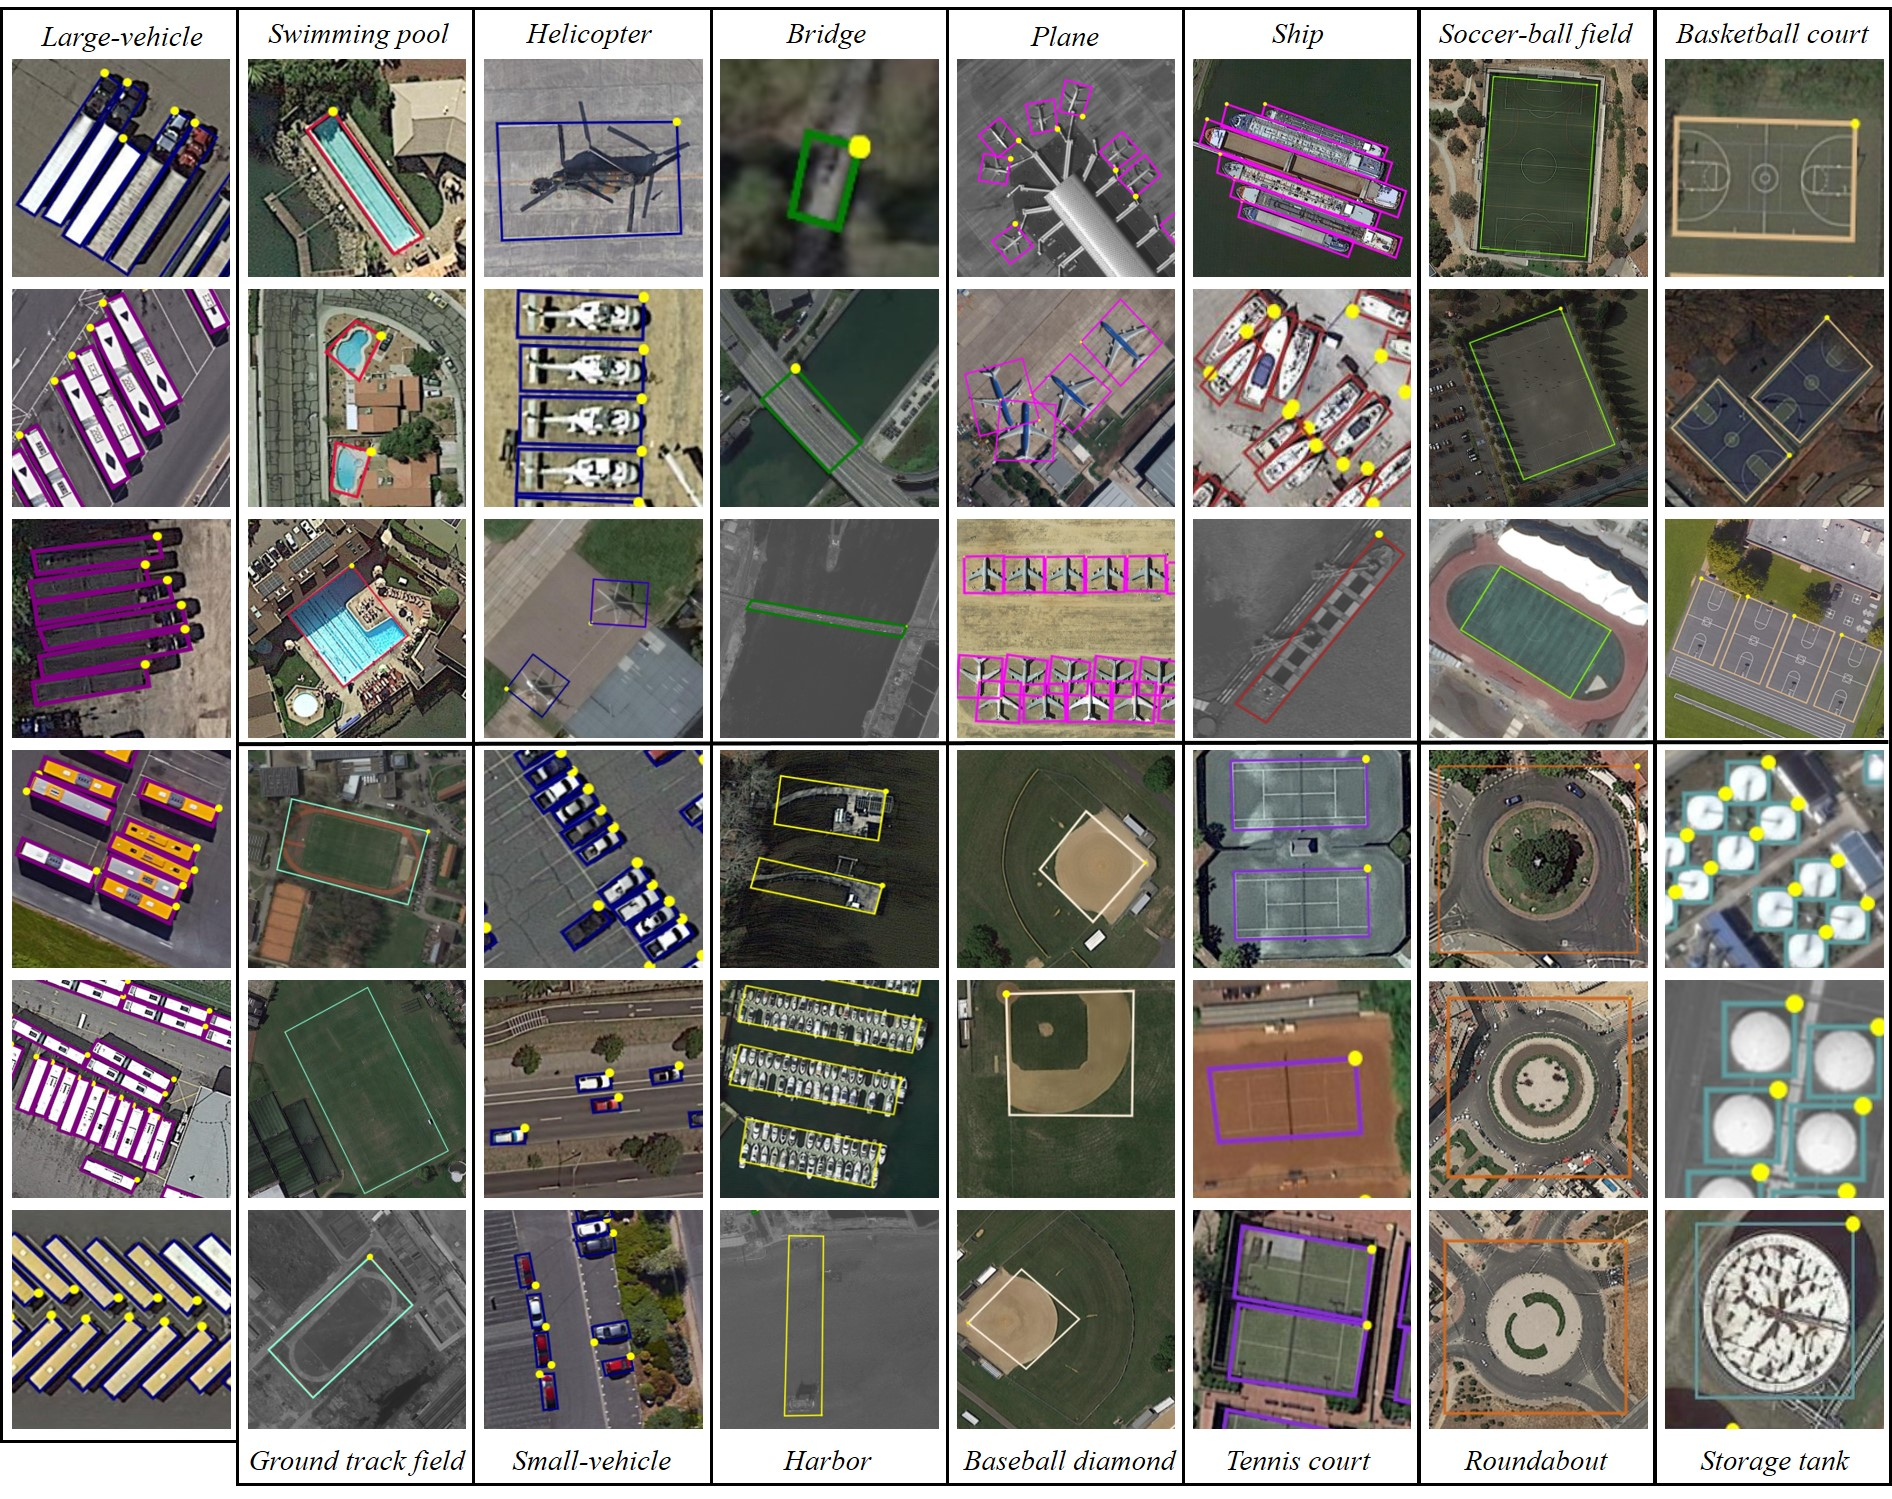
\includegraphics[width=0.95\linewidth]{instances-DOTA.jpg}
\end{center}
\vspace{-3mm}
\caption{Samples of annotated images in the competition. We show three samples per each category, except six for {\em large-vehicle}. }
\label{fig:samples}
\vspace{-2mm}
\end{figure*}

\section{Tasks of competition}
\subsection{Task 1 - Detection with horizontal bounding boxes }
Detecting object with horizontal bounding boxes is usual in many previous competitions for object detection. The aim of this task is to accurately localize the instance in terms of horizontal bounding box with $(x, y, w, h)$ format. In the task, the ground truths for training and testing are generated by calculating the axis-aligned bounding boxes over original annotated bounding boxes.
\subsubsection*{Submission Format}
Participants will be asked to submit a zip file containing results for all test images. The results format is:

$$x^{(1)}, y^{(1)}, w^{(1)}, h^{(1)},  category, score$$
$$x^{(2)}, y^{(2)}, w^{(2)}, h^{(2)},  category, score$$
$$...$$
\subsubsection*{Evaluation Protocol}
The evaluation protocol for horizontal bounding boxes follows the PASCAL VOC~\cite{PASCALVOC} benchmark, which uses mean Average Precision(map) as the primary metric.

\subsection{Task 2 - Detection with oriented bounding boxes}
The aim of this task is to locate the ground object instances with an oriented bounding box. The oriented bounding box follows the same format with the original annotation $\{(x_i, y_i), i = 1, 2, 3, 4\}$

\subsubsection*{Submission Format}
Participants will be asked to submit a zip file containing results for all test images. The results format is:

$$x_1^{(1)}, y_1^{(1)}, x_2^{(1)}, y_2^{(1)}, x_3^{(1)}, y_3^{(1)}, x_4^{(1)}, y_4^{(1)}, category, score$$
$$x_1^{(2)}, y_1^{(2)}, x_2^{(2)}, y_2^{(2)}, x_3^{(2)}, y_3^{(2)}, x_4^{(2)}, y_4^{(2)}, category, score$$
$$...$$

\subsubsection*{Evaluation Protocol}
The evaluation protocol for oriented bounding box is a little different from the protocol in the original PASCAL VOC. We use the intersection over the union area of two polygons(ground truth and prediction) to calculate the IoU. The rest follows the PASCAL VOC.

\section{Organization}
We will set up a website to maintain information of the competition, download links for the datasets, and user interfaces for participants to register and submit their results. After the submission deadline, we will collect all submissions and evaluate their performance. A winner will be determined for each task based on the score achieved by the corresponding metric.

The expected number of participant is over 30, since more than 50 research teams from top universities (e.g., UC Berkeley, the Chinese University of Hong Kong and Tsinghua University), leading institutions (e.g., Microsoft Research Asia and Institute of Automation of the Chinese Academy of Sciences) and high-tech AI companies (e.g., Facebook, Baidu, SenseTime and Hikvision), from countries around the world, have conducted penetrating research on general object detection in natural images. For the sake of attracting more participants, we are considering inviting industrial sponsors to provide some cash award for the winner of the competition.

All datasets and the evaluation code used in the competition will be made public after the end of the competition.



\section{Organization Team}
\begin{itemize}
\item \textbf{Gui-Song Xia}, Professor at LIESMARS, Wuhan University, China (guisong.xia@whu.edu.cn)
\item \textbf{Fan Hu}, Postdoctoral researcher at the Electronic Information School, Wuhan University, China (fanhu@whu.edu.cn)
\item \textbf{Xiang Bai}, Professor of the School of Electronic Information and Communications, Huazhong University of Science and Technology (xbai@hust.edu.cn)
\item \textbf{Serge Belongie}, Professor at Cornell Tech and the Department of Computer Science at Cornell University, United States (sjb344@cornell.edu )
\item \textbf{Jiebo Luo}, Professor of Computer Science, University of Rochester (jiebo.luo@gmail.com)
\item \textbf{Mihai Datcu}, Scientist with the German
Aerospace Center (DLR) (mihai.datcu@dlr.de)
\item \textbf{Marcello Pelillo}, Professor of Computer Science, Ca' Foscari University of Venice (pelillo@dsi.unive.it)
\item \textbf{Liangpei Zhang}, Professor at LIESMARS, Wuhan University, China (zlp62@whu.edu.cn)
\end{itemize}


\section{Schedule}
\begin{itemize}
	\item Website goes online:												January 31 , 2018
	\item Registration open:													   January 31 - March 31, 2018
	\item Training/Validation dataset available:				February 15, 2018
	\item Test dataset available:											March 15, 2018
	\item Submission open:													  March 15, 2018
	\item Submission deadline:											  April 15, 2018
	\item Submission of competition report:					April 30, 2018
\end{itemize}

\section{Short Bios of the Organizers}
\textbf{Gui-Song Xia} received the
B.S. degree in electronics engineering and the M.S.
degree in signal processing from Wuhan University,
Wuhan, China, in 2005 and 2007, respectively, and
the Ph.D. degree in image processing and computer
vision from the Centre National de la Recherche
Scientifique (CNRS) Laboratoire Traitement et
Communication de l’Information, TELECOM
ParisTech, Paris, France, in 2011.
In 2011, he was a Post-Doctoral Researcher
with the Centre de Recherche en Mathmatiques de
la Decision, CNRS, Paris-Dauphine University, Paris, for one and a half
years. He is currently a Full Professor with the State Key Laboratory of
Information Engineering, Surveying, Mapping and Remote Sensing, Wuhan
University. His research interests include mathematical image modeling,
texture synthesis, image indexing and content-based retrieval, structure from
motion, perceptual grouping, and remote sensing imaging.
\vspace{3mm}

\noindent\textbf{Xiang Bai} received the B.S., M.S., and
Ph.D. degrees from the Huazhong University of
Science and Technology (HUST), Wuhan, China, in
2003, 2005, and 2009, respectively, all in electronics
and information engineering.
He is currently a Professor with the School of
Electronic Information and Communications and
the Vice-Director of the National Center of AntiCounterfeiting
Technology, HUST. His research
interests include object recognition, shape analysis,
and scene text recognition.

\vspace{3mm}
\noindent\textbf{Serge Belongie} received a B.S. (with honor) in EE from Caltech in 1995 and a Ph.D. in EECS from Berkeley in 2000. While at Berkeley, his research was supported by an NSF Graduate
Research Fellowship. From 2001-2013 he was a professor in the Department of Computer
Science and Engineering at University of California, San Diego.
He is currently a professor at Cornell Tech and the Department of Computer Science at Cornell
University. His research interests include Computer Vision, Machine Learning, Crowdsourcing
and Human-in-the-Loop Computing. He is also a co-founder of several companies including
Digital Persona, Anchovi Labs and Orpix. He is a recipient of the NSF CAREER Award, the
Alfred P. Sloan Research Fellowship, the MIT Technology Review “Innovators Under 35”
Award and the Helmholtz Prize for fundamental contributions in Computer Vision.
\vspace{3mm}

\noindent\textbf{Jiebo Luo} joined the
Department of Computer Science, University of
Rochester, in 2011, after a prolific career of over
15 years with Kodak Research. He has authored
over 300 technical papers. He holds 90 U.S. patents.
His research interests include the computer vision,
machine learning, data mining, social media, and
biomedical informatics. He is a fellow of the SPIE and the IAPR.
\vspace{3mm}

\noindent\textbf{Mihai Datcu} received the M.S. and Ph.D. degrees
in electronics and telecommunications from the University
“Politehnica” of Bucharest UPB, Bucharest,
Romania, in 1978 and 1986, and the title “Habilitation
a diriger des recherches” from Université Louis
Pasteur, Strasbourg, France.
He holds a Professorship in electronics and
telecommunications with UPB since 1981. Since
1993, he has been a Scientist with the German
Aerospace Center (DLR), Oberpfaffenhofen,
Germany. He is currently developing algorithms
for model-based information retrieval from high-complexity signals, methods
for scene understanding from SAR and interferometric SAR data, and he is
engaged in research in information theoretical aspects and semantic representations
in advanced communication systems. His research interests are in Bayesian inference, information and complexity
theory, stochastic processes, model-based scene understanding, image
information mining, for applications in information retrieval and understanding
of high-resolution SAR and optical observations.
\vspace{3mm}

\noindent\textbf{Marcello Pelillo } is a Professor
of Computer Science at Ca’ Foscari University of
Venice, Italy, where he directs the European Centre
for Living Technology (ECLT). He held visiting
research positions at Yale University, McGill University,
the University of Vienna, York University
(U.K.), the University College London, and the
National ICT Australia (NICTA). He has published
more than 200 technical papers in refereed journals,
handbooks, and conference proceedings in the areas
of machine learning, computer vision, and pattern
recognition.
Prof. Pelillo is a fellow of the IAPR. He has recently been appointed
as IEEE SMC Distinguished Lecturer.
\vspace{3mm}

\noindent\textbf{Fan Hu } received the B.S. degree in communication
engineering from Wuhan University,
Wuhan, China, in 2011, where he is currently a postdoctoral researcher at the Electronic Information School, Wuhan University, China.
His research interests include high-resolution
image classification, and machine learning, especially
deep learning and their applications in remote
sensing.
\vspace{3mm}

\noindent\textbf{Liangpei Zhang} received the B.S.
degree in physics from Hunan Normal University,
Changsha, China, in 1982, the M.S. degree in optics
from the Xi’an Institute of Optics and Precision
Mechanics, Chinese Academy of Sciences, Xi’an,
China, in 1988, and the Ph.D. degree in photogrammetry
and remote sensing from Wuhan University,
Wuhan, China, in 1998. He is currently the
Head of the Remote Sensing Division, State Key Laboratory of Information
Engineering in Surveying, Mapping, and Remote Sensing, Wuhan University.
He is also a Chang-Jiang Scholar Chair Professor appointed by the Ministry of
Education of China. He has authored over 500 research papers and five books. His research interests include hyperspectral remote
sensing, high-resolution remote sensing, image processing, and artificial
intelligence.
Dr. Zhang is a fellow of the Institution of Engineering and Technology, an
Executive Member (Board of Governor) of the China National Committee of
International Geosphere–Biosphere Programme, and an Executive Member of
the China Society of Image and Graphics. He was
a recipient of the 2010 Best Paper Boeing Award and the 2013 Best Paper
ERDAS Award from the American Society of Photogrammetry and Remote
Sensing. He is currently
serving as an Associate Editor of the IEEE TRANSACTIONS ON GEOSCIENCE
AND REMOTE SENSING.

{\small
\bibliographystyle{ieee}
%\bibliography{egbib}
\bibliography{aerial_detection_dataset}
}

\end{document}